\documentclass[a4paper, 12pt]{article}
\usepackage[a4paper,top=1.5cm, bottom=1.5cm, left=1cm, right=1cm]{geometry}

% Работа с русским языком
\usepackage[utf8]{inputenc}
\usepackage{mathtext}                % русские буквы в формулах
\usepackage[english, russian]{babel} % локализация и переносы

\usepackage{graphicx}   % Вставка изображений
\usepackage{float}      % "Плавающие" изображения3
\usepackage{wrapfig}    % Обтекание фигур (таблиц, картинок и прочего)
\graphicspath{ {./images/} }

\usepackage{tabularx}
\usepackage{multirow}
\usepackage{amsmath}
\usepackage{amsfonts}
\usepackage{indentfirst}
\usepackage{longtable}
\graphicspath{{pictures/}}
\usepackage{natbib}

%%% Колонтитулы
\usepackage{titleps}
\newpagestyle{main}{
	\setheadrule{0.4pt}
	\sethead{Отчёт о выполнении лабораторной работы 2.5.1}{}{}
	\setfootrule{0.4pt}                       
	\setfoot{ФРКТ МФТИ, 2023}{}{\thepage} 
}
\pagestyle{main}  

\begin{document}
    \begin{titlepage}
	\begin{center}
            {\large МОСКОВСКИЙ ФИЗИКО-ТЕХНИЧЕСКИЙ ИНСТИТУТ (НАЦИОНАЛЬНЫЙ       ИССЛЕДОВАТЕЛЬСКИЙ УНИВЕРСИТЕТ)}
	\end{center}
 
	\begin{center}
		{\large Физтех-школа радиотехники и компьютерных технологий}
	\end{center}
	
	\vspace{8cm}
	{\LARGE
		\begin{center}
                {\bf Отчёт о выполнении лабораторной работы 2.5.1}\\
                Измерение коэффициента поверхностного натяжения жидкости
		\end{center}
	}
	\vspace{5cm}
	\begin{flushright}
		{\Large Автор:\\ Тихонов Дмитрий Романович, \\
			\vspace{0.2cm}
			студент группы Б01-206}
	\end{flushright}
	\vspace{5cm}
	\begin{center}
		\Large Долгопрудный, 2023
	\end{center}
    \end{titlepage}

    \section*{Введение}

    \noindent \textbf{Цель работы:}  
    \begin{enumerate}
        \item измерение температурной зависимости  коэффициента поверхностного натяжения дистиллированной воды с использованием известного коэффициента поверхностного натяжения спирта;
        \item определение полной поверхностной энергии  и теплоты, необходимой для изотермического образования единицы  поверхности жидкости  при различной температуре.
    \end{enumerate}

    \noindent \textbf{В работе используются:} прибор  Ребиндера  с термостатом и микроманометром; исследуемые жидкости; стаканы; микроскоп.
    
    \section*{Теоретические сведения}

        \noindent Наличие поверхностного слоя приводит к различию давлений по разные стороны от искривленной границы раздела двух сред.  Для сферического пузырька с воздухом  внутри жидкости избыточное давление даётся формулой Лапласа:

        \begin{equation}
            \label{key}
            \Delta P = P_{int} - P_{ext} = \frac{2\sigma}{r},
        \end{equation}
        \noindent где $\sigma$ -- коэффициент поверхностного натяжения, $P_{int}$ и $P_{ext}$ -- давление внутри пузырька и снаружи, $r$ -- радиус кривизны поверхности раздела двух фаз. Эта формула лежит в основе предлагаемого метода определения коэффициента поверхностного натяжения жидкости. Измеряется давление $\Delta P$, необходимое для выталкивания в жидкость пузырька воздуха.

    \section*{Методика измерений и используемое оборудование}

    \begin{figure}[H]
        \centering
        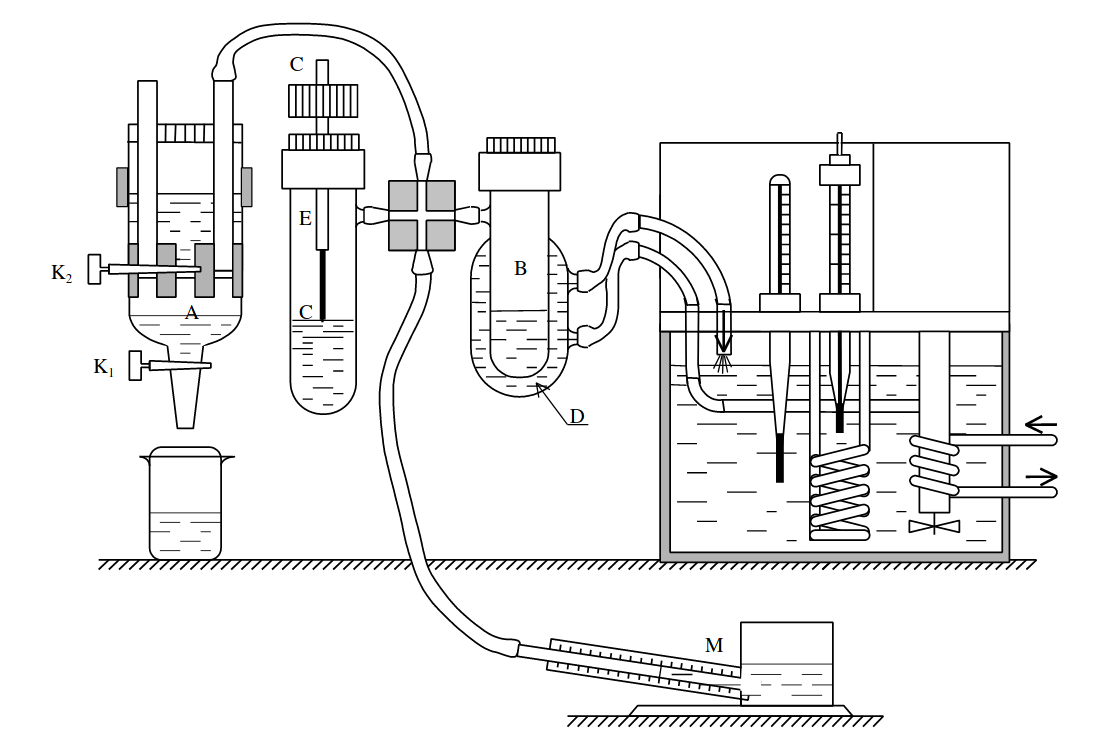
\includegraphics[width=15cm]{images/installation.png}
        \caption{Рисунок экспериментальной установки}
        \label{img:ust}
    \end{figure}

    \noindent Исследуемая жидкость (дистиллированная вода) наливается в сосуд (колбу) $ B $ (рис. \ref{img:ust}). Тестовая жидкость  (этиловый спирт) наливается  в сосуд $ E $.  При измерениях  колбы герметично закрываются  пробками. Через одну из двух пробок  проходит полая металлическая игла $ С $. Этой пробкой закрывается сосуд, в котором  проводятся измерения. Верхний конец иглы открыт в атмосферу, а нижний погружен в жидкость. Другой сосуд герметично закрывается второй пробкой. При создании достаточного  разряжения воздуха в колбе с иглой пузырьки воздуха начинают пробулькивать через жидкость. Поверхностное натяжение можно определить по величине разряжения $ \Delta P $ \eqref{key}, необходимого для прохождения пузырьков (при известном радиусе иглы). \\

    \noindent Разряжение в системе создается с помощью аспиратора $ A $. Кран $ K_2 $ разделяет две полости аспиратора. Верхняя полость при закрытом кране $ K_2 $ заполняется водой. Затем кран $ K_2 $ открывают и заполняют водой  нижнюю полость  аспиратора.  Разряжение воздуха создается в нижней полости  при открывании крана $ K_1 $, когда  вода вытекает из неё по каплям. В колбах $ В $ и $ С $, соединённых трубками с нижней полостью аспиратора, создается такое же пониженное давление. Разность давлений в полостях с разряженным воздухом и атмосферой измеряется спиртовым микроманометром.\\

    \noindent Для стабилизации температуры исследуемой жидкости через рубашку $ D $ колбы $ В $ непрерывно прогоняется вода из термостата.\\

    \noindent Обычно кончик иглы лишь касается поверхности жидкости, чтобы исключить влияние гидростатического давления столба жидкости. Однако при измерении температурной зависимости коэффициента поверхностного натяжения возникает ряд сложностей. Во-первых, большая теплопроводность металлической трубки приводит к тому, что температура на конце трубки заметно ниже, чем в глубине жидкости. Во-вторых, тепловое расширение поднимает уровень жидкости при увеличении температуры.\\

    \noindent Обе погрешности можно устранить, погрузив кончик трубки до самого дна. Полное давление, измеренное при этом микроманометром, равно \[ P = \Delta P + \rho g h.\] Заметим, что $ \rho gh $ от температуры практически не зависит, так как подъём уровня жидкости компенсируется уменьшением её плотности (произведение $ \rho g $ определяется массой всей жидкости и поэтому постоянно). Величину  $ \rho g h $ следует измерить двумя способами.\\

    \noindent Во-первых, замерить величину $P_1= \Delta P'$, когда кончик трубки только касается поверхности жидкости. Затем при этой же температуре опустить иглу до дна и замерить $P_2= \rho gh + \Delta P''$ ($\Delta P'$, $\Delta P''$ -- давление Лапласа). Из-за  несжимаемости  жидкости можно положить $\Delta P' = \Delta P''$ и тогда \[ \rho gh= P_2 - P_1. \]
 
    \noindent Во-вторых, при измерениях $P_1$ и $P_2$ замерить линейкой  глубину погружения иглы $h$. Это можно сделать, замеряя расстояние между верхним концом иглы и любой неподвижной частью прибора при положении иглы на поверхности и в глубине колбы.    

    \section*{Результаты измерений и обработка данных}

    \subsection*{Измерение диаметра иглы}

    \noindent Измерим максимальное давление $\Delta P_{alc}$  при  пробулькивании пузырьков воздуха через спирт. Результаты измерений занесём в таблицу \ref{tab:alcohol}.

    \begin{table}[H]
	\centering
	\begin{tabular}{|c|c|c|c|c|}
		\hline
            № & $ P' $, дел. &  $ P $, Па  & $ \langle P \rangle $, Па   & $ \sigma_{P} $, Па \\ \hline
            1 & 47 & 92,21 & \multirow{10}{*}{90,6} & \multirow{10}{*}{2,0} \\ \cline{1-3}
            2  & 46 & 90,25 & & \\ \cline{1-3}
            3  & 46 & 90,25 & & \\ \cline{1-3}
            4  & 46 & 90,25 & & \\ \cline{1-3}
            5  & 46 & 90,25 & & \\ \cline{1-3}
            6  & 46 & 90,25 & & \\ \cline{1-3}
            7  & 46 & 90,25 & & \\ \cline{1-3}
            8  & 46 & 90,25 & & \\ \cline{1-3}
            9  & 47 & 92,21 & & \\ \cline{1-3}
            10 & 46 & 90,25 & & \\ \hline
	\end{tabular}
	\caption{Результаты измерений в спирте}
	\label{tab:alcohol}
    \end{table}

    \noindent Учтём, что показания микроманометра связаны с давлением следующим соотношением: \[ P=P' \cdot 0,2 \cdot 9,81, \] где $P'$ -- количество делений шкалы, а константы остаются постоянными во время всей работы и определяются исходя из паспорта устройства.\\

    \noindent Вычислим среднее значение измеренного давления. Для этого воспользуемся следующей формулой:

    \begin{equation}
        \label{mid}
        \langle P \rangle = \frac{\sum\limits_{k=1}^{N} P_k}{N} \approx 90,6 \text{ Па},
    \end{equation}
    \noindent где $ N $ -- число проведённых измерений.\\

    \noindent Также вычислим случайную погрешность измерений по формуле

    \begin{equation}\label{occasion}
        \sigma_{P}^{\text{случ}} = \sqrt{\frac{1}{N(N-1)}\sum\limits_{k=1}^N\left(P_k-\langle P \rangle\right)^2} \approx 0,6 \text{ Па}.
    \end{equation}
    
    \noindent Систематическую погрешность определим из расчёта, что погрешность измерения составила $1$ деление прибора, или же \underline{$\sigma_{P}^\text{сист} \approx 2,0$ Па}.\\

    \noindent Полная погрешность измерений определяется по формуле:

    \begin{equation}
        \label{full_pogr}
        \sigma_{P}=\sqrt{(\sigma_{P}^\text{сист})^2 + (\sigma_{P}^\text{случ})^2} \approx 2,0 \text{ Па}.
    \end{equation}

    \noindent Итого получаем \underline{ $\Delta P_{alc} = (90,6 \pm 2,0) \text{ Па},$}\quad $(\varepsilon = 2,2 \%) $. \\

    \noindent Согласно ГОСТ 8.428-81 коэффициент поверхностного натяжения этилового спирта при комнатной температуре равен $ \sigma_{alc} = 22,4 $ мН/м. По полученным результатам измерения и при помощи \eqref{key} вычисляем диаметр иглы по формуле:

    \begin{equation}
        \label{igla}
        d=\frac{4\sigma_{alc}}{\Delta P_{alc}} \approx 0,99 \text{ мм}.
    \end{equation}

    \noindent Также вычисляем погрешность полученного результата:

    \begin{equation}
        \label{igla_pogr}
        \sigma_d=d\cdot\varepsilon_{\Delta P_{alc}} \approx 0,02 \text{ мм}.
    \end{equation}

    \noindent Таким образом, получаем окончательный результат измерения диаметра иглы косвенным способом:
    $$\boxed{ d = (0,99 \pm 0,02) \text{ мм}} \: (\varepsilon = 2,2\%).$$

    \noindent Также проведём измерение диаметра иглы при помощи оптического микроскопа (см. рис.~\ref{img:igla}).

    \begin{figure}[H]
        \centering
        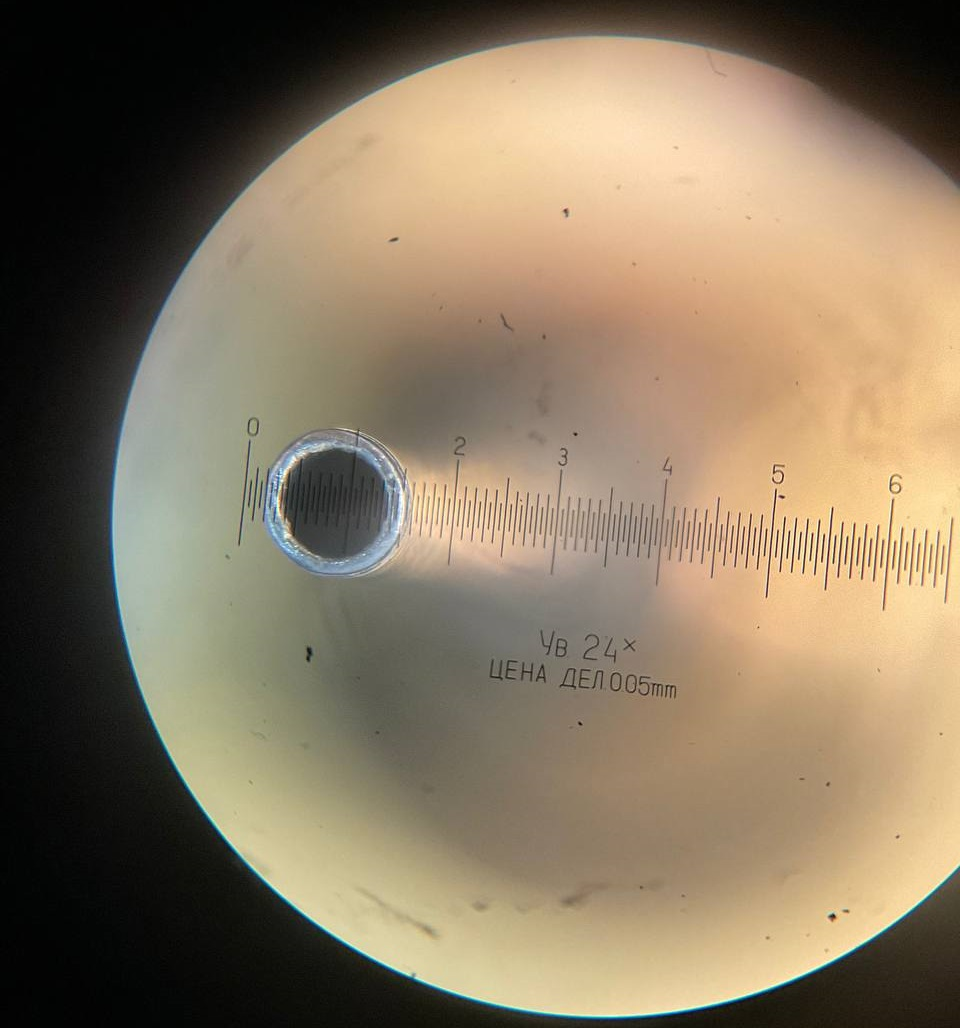
\includegraphics[width=16cm]{images/spine.jpeg}
        \caption{Измерение диаметра иглы при помощи оптического микроскопа}
        \label{img:igla}
    \end{figure}

    \noindent По результатам прямого измерения получаем $ \underline{d = (1,00 \pm 0,05) \text{ мм}}, \: (\varepsilon = 5\%) $.\\

    \noindent Таким образом, диаметр иглы, измеренный двумя различными способами, совпадает в пределах погрешности, что может говорить о справедливости формулы, представленной в теоретических сведениях, а также об исправной работе экспериментальной установки.

    \subsection*{Определение поправки при измерении давления для погруженной в воду иглы}

    \noindent Перенесём предварительно промытую и просушенную от спирта иглу в колбу с дистиллированной водой. Измерим максимальное давление $P_1$ при пробулькивании пузырьков, когда игла лишь касается поверхности воды. Измерим расстояние между верхним концом иглы и любой неподвижной часть прибора $h_1$. \\

    \noindent После этого, утопим иглу в воду. Измерим $h_2$. Также измерим максимальное давление в пузырьках $P_2$. Полученные результаты заносим в таблицу \ref{tab:popravka}.

    \begin{table}[H]
    	\centering
    	\begin{tabular}{ccccccc}
    		\hline
    		\multicolumn{1}{|c|}{№} &
    		\multicolumn{1}{c|}{$ P_1 $, дел.} &
    		\multicolumn{1}{c|}{$ P_1 $, Па} &
    		\multicolumn{1}{c|}{$ \langle P_1 \rangle $, Па} &
    		\multicolumn{1}{c|}{$ \sigma_{P_1} $, Па} &
    		\multicolumn{1}{c|}{$ h_1 $, мм} &
    		\multicolumn{1}{c|}{$ \sigma_{h_1} $, мм} \\ \hline
                \multicolumn{1}{|c|}{1} & \multicolumn{1}{c|}{140} & \multicolumn{1}{c|}{274,68} & \multicolumn{1}{c|}{\multirow{10}{*}{276,2}} & \multicolumn{1}{c|}{\multirow{10}{*}{2,0}} & \multicolumn{1}{c|}{\multirow{10}{*}{18,0}} & \multicolumn{1}{c|}{\multirow{10}{*}{0,5}} \\ \cline{1-3}
                \multicolumn{1}{|c|}{2}     & \multicolumn{1}{c|}{141} & \multicolumn{1}{c|}{276,64} & \multicolumn{1}{c|}{} & \multicolumn{1}{c|}{} & \multicolumn{1}{c|}{} & \multicolumn{1}{c|}{} \\ \cline{1-3}
                \multicolumn{1}{|c|}{3} & \multicolumn{1}{c|}{141} & \multicolumn{1}{c|}{276,64} & \multicolumn{1}{c|}{} & \multicolumn{1}{c|}{} & \multicolumn{1}{c|}{} & \multicolumn{1}{c|}{} \\ \cline{1-3}
                \multicolumn{1}{|c|}{4} & \multicolumn{1}{c|}{141} & \multicolumn{1}{c|}{276,64} & \multicolumn{1}{c|}{} & \multicolumn{1}{c|}{} & \multicolumn{1}{c|}{} & \multicolumn{1}{c|}{} \\ \cline{1-3}
                \multicolumn{1}{|c|}{5} & \multicolumn{1}{c|}{140} & \multicolumn{1}{c|}{274,68} & \multicolumn{1}{c|}{} & \multicolumn{1}{c|}{} & \multicolumn{1}{c|}{} & \multicolumn{1}{c|}{} \\ \cline{1-3}
                \multicolumn{1}{|c|}{6} & \multicolumn{1}{c|}{141} & \multicolumn{1}{c|}{276,64} & \multicolumn{1}{c|}{} & \multicolumn{1}{c|}{} & \multicolumn{1}{c|}{} & \multicolumn{1}{c|}{} \\ \cline{1-3}
                \multicolumn{1}{|c|}{7} & \multicolumn{1}{c|}{141} & \multicolumn{1}{c|}{276,64} & \multicolumn{1}{c|}{} & \multicolumn{1}{c|}{} & \multicolumn{1}{c|}{} & \multicolumn{1}{c|}{} \\ \cline{1-3}
                \multicolumn{1}{|c|}{8} & \multicolumn{1}{c|}{141} & \multicolumn{1}{c|}{276,64} & \multicolumn{1}{c|}{} & \multicolumn{1}{c|}{} & \multicolumn{1}{c|}{} & \multicolumn{1}{c|}{} \\ \cline{1-3}
                \multicolumn{1}{|c|}{9} & \multicolumn{1}{c|}{141} & \multicolumn{1}{c|}{276,64} & \multicolumn{1}{c|}{} & \multicolumn{1}{c|}{} & \multicolumn{1}{c|}{} & \multicolumn{1}{c|}{} \\ \cline{1-3}
                \multicolumn{1}{|c|}{10} & \multicolumn{1}{c|}{141} & \multicolumn{1}{c|}{276,64} & \multicolumn{1}{c|}{} & \multicolumn{1}{c|}{} & \multicolumn{1}{c|}{} & \multicolumn{1}{c|}{} \\ \hline
    		&
    		&
    		&
    		&
    		&
    		&
    		\\ \hline
    		\multicolumn{1}{|c|}{№} &
    		\multicolumn{1}{c|}{$ P_2 $, дел.} &
    		\multicolumn{1}{c|}{$ P_2 $, Па} &
    		\multicolumn{1}{c|}{$ \langle P_2 \rangle $, Па} &
    		\multicolumn{1}{c|}{$ \sigma_{P_2} $, Па} &
    		\multicolumn{1}{c|}{$ h_2 $, мм} &
    		\multicolumn{1}{c|}{$ \sigma_{h_2} $, мм} \\ \hline
                \multicolumn{1}{|c|}{1} & \multicolumn{1}{c|}{204} & \multicolumn{1}{c|}{400,25} & \multicolumn{1}{c|}{\multirow{10}{*}{400,6}} & \multicolumn{1}{c|}{\multirow{10}{*}{2,0}} & \multicolumn{1}{c|}{\multirow{10}{*}{5,0}} & \multicolumn{1}{c|}{\multirow{10}{*}{0,5}} \\ \cline{1-3}
                \multicolumn{1}{|c|}{2} & \multicolumn{1}{c|}{205} & \multicolumn{1}{c|}{402,21} & \multicolumn{1}{c|}{} & \multicolumn{1}{c|}{} & \multicolumn{1}{c|}{} & \multicolumn{1}{c|}{} \\ \cline{1-3}
                \multicolumn{1}{|c|}{3} & \multicolumn{1}{c|}{204} & \multicolumn{1}{c|}{400,25} & \multicolumn{1}{c|}{} & \multicolumn{1}{c|}{} & \multicolumn{1}{c|}{} & \multicolumn{1}{c|}{} \\ \cline{1-3}
                \multicolumn{1}{|c|}{4} & \multicolumn{1}{c|}{205} & \multicolumn{1}{c|}{402,21} & \multicolumn{1}{c|}{} & \multicolumn{1}{c|}{} & \multicolumn{1}{c|}{} & \multicolumn{1}{c|}{} \\ \cline{1-3}
                \multicolumn{1}{|c|}{5} & \multicolumn{1}{c|}{204} & \multicolumn{1}{c|}{400,25} & \multicolumn{1}{c|}{} & \multicolumn{1}{c|}{} & \multicolumn{1}{c|}{} & \multicolumn{1}{c|}{} \\ \cline{1-3}
                \multicolumn{1}{|c|}{6} & \multicolumn{1}{c|}{204} & \multicolumn{1}{c|}{400,25} & \multicolumn{1}{c|}{} & \multicolumn{1}{c|}{} & \multicolumn{1}{c|}{} & \multicolumn{1}{c|}{} \\ \cline{1-3}
                \multicolumn{1}{|c|}{7} & \multicolumn{1}{c|}{204} & \multicolumn{1}{c|}{400,25} & \multicolumn{1}{c|}{} & \multicolumn{1}{c|}{} & \multicolumn{1}{c|}{} & \multicolumn{1}{c|}{} \\ \cline{1-3}
                \multicolumn{1}{|c|}{8} & \multicolumn{1}{c|}{204} & \multicolumn{1}{c|}{400,25} & \multicolumn{1}{c|}{} & \multicolumn{1}{c|}{} & \multicolumn{1}{c|}{} & \multicolumn{1}{c|}{} \\ \cline{1-3}
                \multicolumn{1}{|c|}{9} & \multicolumn{1}{c|}{204} & \multicolumn{1}{c|}{400,25} & \multicolumn{1}{c|}{} & \multicolumn{1}{c|}{} & \multicolumn{1}{c|}{} & \multicolumn{1}{c|}{} \\ \cline{1-3}
                \multicolumn{1}{|c|}{10} & \multicolumn{1}{c|}{204} & \multicolumn{1}{c|}{400,25} & \multicolumn{1}{c|}{} & \multicolumn{1}{c|}{} & \multicolumn{1}{c|}{} & \multicolumn{1}{c|}{} \\ \hline
    	\end{tabular}
    	\caption{Определение поправки к давлению}
    	\label{tab:popravka}
    \end{table}

    \noindent Исходя из экспериментальных данных, определяем среднее значение давления $\langle P \rangle$ и погрешность измерения $\sigma_{P}$ по формулам \eqref{mid}, \eqref{occasion} и \eqref{full_pogr}.\\

    \noindent По полученным данным определяем \[ P_2-P_1 = 124,4 \text{ Па}. \]

    \noindent Также вычисляем погрешность:  
    \begin{equation}
        \label{pogr_sum}
        \sigma_{\Delta P} = \sqrt{\sigma^2_{P_1}+\sigma^2_{P_2}} \approx 2,8 \text{ Па}.
    \end{equation}

    \noindent Таким образом, получаем $\underline{\Delta P = (124,4 \pm 2,8) \text{ Па},} \: (\varepsilon = 2,3\%).$\\

    \noindent По полученному значению $\Delta P$ можем рассчитать $\Delta h$ по следующей формуле: \[ \Delta h = \frac{\Delta P}{\rho g} \approx 12,7 \text{ мм}, \] где $ \rho = 1000 $ кг/$ \text{м}^3 $ -- плотность воды и $g = 9,81$ м/$\text{с}^2$ -- ускорение свободного падения.\\
    
    \noindent При этом погрешность нашего измерения равна \[ \sigma_{\Delta h} = \Delta h \cdot \varepsilon_{\Delta P} \approx 0,3 \text{ мм}. \]

    \noindent Таким образом, получаем $\underline{\Delta h = (12,7 \pm 0,3) \text{ мм}}, \: (\varepsilon = 2,3\%).$\\
    
    \noindent Заметим, что полученный результат в пределах погрешности совпадает с результатом, полученном прямым измерением $ \underline{\Delta h' = (13,0 \pm 0,7) \text{ мм},} \: (\varepsilon = 5,4\%). $\\

    \noindent Значит, в ходе дальнейших измерений мы будем делать поправку \label{popravka} $  \underline{\Delta P = (124,4 \pm 2,8) \text{ Па},}$ на~добавочное давление со стороны столба жидкости.

    \subsection*{Измерение температурной зависимости коэффициента поверхностного натяжения}
  
    \noindent Снимем температурную зависимость $\sigma(T)$ дистиллированной воды. Для этого включим термостат и подождём, пока нужная нам температура не стабилизируется. После этого проведём измерение давления. Для уменьшения погрешности опыта замер давления  при фиксированной температуре проведём несколько раз. Результаты измерений занесём в таблицу \ref{tab:pov}.
    
    \begin{table}[H]
    	\centering
    	\begin{tabular}{ccccccc}
    		\hline
    		\multicolumn{1}{|c|}{$ T $, К} &
    		\multicolumn{1}{c|}{$ P' $, дел} &
    		\multicolumn{1}{c|}{$ P' $, Па} &
    		\multicolumn{1}{c|}{$ \langle P' \rangle $, Па} &
    		\multicolumn{1}{c|}{$ \sigma_{P'} $, Па} &
    		\multicolumn{1}{c|}{$ P $, Па} &
    		\multicolumn{1}{c|}{$ \sigma_P $, Па} \\ \hline
                \multicolumn{1}{|c|}{\multirow{10}{*}{303,2}} & \multicolumn{1}{c|}{204} & \multicolumn{1}{c|}{400,25} & \multicolumn{1}{c|}{\multirow{10}{*}{398,7}} & \multicolumn{1}{c|}{\multirow{10}{*}{2,0}} & \multicolumn{1}{c|}{\multirow{10}{*}{274,3}} & \multicolumn{1}{c|}{\multirow{10}{*}{3,4}} \\ \cline{2-3}
                \multicolumn{1}{|c|}{} & \multicolumn{1}{c|}{204} & \multicolumn{1}{c|}{400,25} & \multicolumn{1}{c|}{} & \multicolumn{1}{c|}{} & \multicolumn{1}{c|}{} & \multicolumn{1}{c|}{} \\ \cline{2-3}
                \multicolumn{1}{|c|}{} & \multicolumn{1}{c|}{203} & \multicolumn{1}{c|}{398,29} & \multicolumn{1}{c|}{} & \multicolumn{1}{c|}{} & \multicolumn{1}{c|}{} & \multicolumn{1}{c|}{} \\ \cline{2-3}
                \multicolumn{1}{|c|}{} & \multicolumn{1}{c|}{203} & \multicolumn{1}{c|}{398,29} & \multicolumn{1}{c|}{} & \multicolumn{1}{c|}{} & \multicolumn{1}{c|}{} & \multicolumn{1}{c|}{} \\ \cline{2-3}
                \multicolumn{1}{|c|}{} & \multicolumn{1}{c|}{203} & \multicolumn{1}{c|}{398,29} & \multicolumn{1}{c|}{} & \multicolumn{1}{c|}{} & \multicolumn{1}{c|}{} & \multicolumn{1}{c|}{} \\ \cline{2-3}
                \multicolumn{1}{|c|}{} & \multicolumn{1}{c|}{203} & \multicolumn{1}{c|}{398,29} & \multicolumn{1}{c|}{} & \multicolumn{1}{c|}{} & \multicolumn{1}{c|}{} & \multicolumn{1}{c|}{} \\ \cline{2-3}
                \multicolumn{1}{|c|}{} & \multicolumn{1}{c|}{203} & \multicolumn{1}{c|}{398,29} & \multicolumn{1}{c|}{} & \multicolumn{1}{c|}{} & \multicolumn{1}{c|}{} & \multicolumn{1}{c|}{} \\ \cline{2-3}
                \multicolumn{1}{|c|}{} & \multicolumn{1}{c|}{203} & \multicolumn{1}{c|}{398,29} & \multicolumn{1}{c|}{} & \multicolumn{1}{c|}{} & \multicolumn{1}{c|}{} & \multicolumn{1}{c|}{} \\ \cline{2-3}
                \multicolumn{1}{|c|}{} & \multicolumn{1}{c|}{203} & \multicolumn{1}{c|}{398,29} & \multicolumn{1}{c|}{} & \multicolumn{1}{c|}{} & \multicolumn{1}{c|}{} & \multicolumn{1}{c|}{} \\ \cline{2-3}
                \multicolumn{1}{|c|}{} & \multicolumn{1}{c|}{203} & \multicolumn{1}{c|}{398,29} & \multicolumn{1}{c|}{} & \multicolumn{1}{c|}{} & \multicolumn{1}{c|}{} & \multicolumn{1}{c|}{} \\ \hline
    		&
    		&
    		&
    		&
    		&
    		&
    		\\ \hline
    		\multicolumn{1}{|c|}{$ T $, К} &
    		\multicolumn{1}{c|}{$ P' $, дел} &
    		\multicolumn{1}{c|}{$ P' $, Па} &
    		\multicolumn{1}{c|}{$ \langle P' \rangle $, Па} &
    		\multicolumn{1}{c|}{$ \sigma_{P'} $, Па} &
    		\multicolumn{1}{c|}{$ P $, Па} &
    		\multicolumn{1}{c|}{$ \sigma_P $, Па} \\ \hline
                \multicolumn{1}{|c|}{\multirow{10}{*}{308,2}} & \multicolumn{1}{c|}{201} & \multicolumn{1}{c|}{394,36} & \multicolumn{1}{c|}{\multirow{10}{*}{394,6}} & \multicolumn{1}{c|}{\multirow{10}{*}{2,0}} & \multicolumn{1}{c|}{\multirow{10}{*}{270,2}} & \multicolumn{1}{c|}{\multirow{10}{*}{3,4}} \\ \cline{2-3}
                \multicolumn{1}{|c|}{} & \multicolumn{1}{c|}{201} & \multicolumn{1}{c|}{394,36} & \multicolumn{1}{c|}{} & \multicolumn{1}{c|}{} & \multicolumn{1}{c|}{} & \multicolumn{1}{c|}{} \\ \cline{2-3}
                \multicolumn{1}{|c|}{} & \multicolumn{1}{c|}{201} & \multicolumn{1}{c|}{394,36} & \multicolumn{1}{c|}{} & \multicolumn{1}{c|}{} & \multicolumn{1}{c|}{} & \multicolumn{1}{c|}{} \\ \cline{2-3}
                \multicolumn{1}{|c|}{} & \multicolumn{1}{c|}{201} & \multicolumn{1}{c|}{394,36} & \multicolumn{1}{c|}{} & \multicolumn{1}{c|}{} & \multicolumn{1}{c|}{} & \multicolumn{1}{c|}{} \\ \cline{2-3}
                \multicolumn{1}{|c|}{} & \multicolumn{1}{c|}{201} & \multicolumn{1}{c|}{394,36} & \multicolumn{1}{c|}{} & \multicolumn{1}{c|}{} & \multicolumn{1}{c|}{} & \multicolumn{1}{c|}{} \\ \cline{2-3}
                \multicolumn{1}{|c|}{} & \multicolumn{1}{c|}{201} & \multicolumn{1}{c|}{394,36} & \multicolumn{1}{c|}{} & \multicolumn{1}{c|}{} & \multicolumn{1}{c|}{} & \multicolumn{1}{c|}{} \\ \cline{2-3}
                \multicolumn{1}{|c|}{} & \multicolumn{1}{c|}{201} & \multicolumn{1}{c|}{394,36} & \multicolumn{1}{c|}{} & \multicolumn{1}{c|}{} & \multicolumn{1}{c|}{} & \multicolumn{1}{c|}{} \\ \cline{2-3}
                \multicolumn{1}{|c|}{} & \multicolumn{1}{c|}{201} & \multicolumn{1}{c|}{394,36} & \multicolumn{1}{c|}{} & \multicolumn{1}{c|}{} & \multicolumn{1}{c|}{} & \multicolumn{1}{c|}{} \\ \cline{2-3}
                \multicolumn{1}{|c|}{} & \multicolumn{1}{c|}{202} & \multicolumn{1}{c|}{396,32} & \multicolumn{1}{c|}{} & \multicolumn{1}{c|}{} & \multicolumn{1}{c|}{} & \multicolumn{1}{c|}{} \\ \cline{2-3}
                \multicolumn{1}{|c|}{} & \multicolumn{1}{c|}{201} & \multicolumn{1}{c|}{394,36} & \multicolumn{1}{c|}{} & \multicolumn{1}{c|}{} & \multicolumn{1}{c|}{} & \multicolumn{1}{c|}{} \\ \hline
    		&
    		&
    		&
    		&
    		&
    		&
    		\\ \hline
    		\multicolumn{1}{|c|}{$ T $, К} &
    		\multicolumn{1}{c|}{$ P' $, дел} &
    		\multicolumn{1}{c|}{$ P' $, Па} &
    		\multicolumn{1}{c|}{$ \langle P' \rangle $, Па} &
    		\multicolumn{1}{c|}{$ \sigma_{P'} $, Па} &
    		\multicolumn{1}{c|}{$ P $, Па} &
    		\multicolumn{1}{c|}{$ \sigma_P $, Па} \\ \hline
                \multicolumn{1}{|c|}{\multirow{10}{*}{313,0}} & \multicolumn{1}{c|}{199} & \multicolumn{1}{c|}{390,44} & \multicolumn{1}{c|}{\multirow{10}{*}{390,8}} & \multicolumn{1}{c|}{\multirow{10}{*}{2,0}} & \multicolumn{1}{c|}{\multirow{10}{*}{266,4}} & \multicolumn{1}{c|}{\multirow{10}{*}{3,4}} \\ \cline{2-3}
                \multicolumn{1}{|c|}{} & \multicolumn{1}{c|}{200} & \multicolumn{1}{c|}{392,40} & \multicolumn{1}{c|}{} & \multicolumn{1}{c|}{} & \multicolumn{1}{c|}{} & \multicolumn{1}{c|}{} \\ \cline{2-3}
                \multicolumn{1}{|c|}{} & \multicolumn{1}{c|}{200} & \multicolumn{1}{c|}{392,40} & \multicolumn{1}{c|}{} & \multicolumn{1}{c|}{} & \multicolumn{1}{c|}{} & \multicolumn{1}{c|}{} \\ \cline{2-3}
                \multicolumn{1}{|c|}{} & \multicolumn{1}{c|}{199} & \multicolumn{1}{c|}{390,44} & \multicolumn{1}{c|}{} & \multicolumn{1}{c|}{} & \multicolumn{1}{c|}{} & \multicolumn{1}{c|}{} \\ \cline{2-3}
                \multicolumn{1}{|c|}{} & \multicolumn{1}{c|}{199} & \multicolumn{1}{c|}{390,44} & \multicolumn{1}{c|}{} & \multicolumn{1}{c|}{} & \multicolumn{1}{c|}{} & \multicolumn{1}{c|}{} \\ \cline{2-3}
                \multicolumn{1}{|c|}{} & \multicolumn{1}{c|}{199} & \multicolumn{1}{c|}{390,44} & \multicolumn{1}{c|}{} & \multicolumn{1}{c|}{} & \multicolumn{1}{c|}{} & \multicolumn{1}{c|}{} \\ \cline{2-3}
                \multicolumn{1}{|c|}{} & \multicolumn{1}{c|}{199} & \multicolumn{1}{c|}{390,44} & \multicolumn{1}{c|}{} & \multicolumn{1}{c|}{} & \multicolumn{1}{c|}{} & \multicolumn{1}{c|}{} \\ \cline{2-3}
                \multicolumn{1}{|c|}{} & \multicolumn{1}{c|}{199} & \multicolumn{1}{c|}{390,44} & \multicolumn{1}{c|}{} & \multicolumn{1}{c|}{} & \multicolumn{1}{c|}{} & \multicolumn{1}{c|}{} \\ \cline{2-3}
                \multicolumn{1}{|c|}{} & \multicolumn{1}{c|}{199} & \multicolumn{1}{c|}{390,44} & \multicolumn{1}{c|}{} & \multicolumn{1}{c|}{} & \multicolumn{1}{c|}{} & \multicolumn{1}{c|}{} \\ \cline{2-3}
                \multicolumn{1}{|c|}{} & \multicolumn{1}{c|}{199} & \multicolumn{1}{c|}{390,44} & \multicolumn{1}{c|}{} & \multicolumn{1}{c|}{} & \multicolumn{1}{c|}{} & \multicolumn{1}{c|}{} \\ \hline
            \end{tabular}
        \end{table}
        
        \begin{table}[H]
    	\centering
    	\begin{tabular}{ccccccc}
                \hline
                \multicolumn{1}{|c|}{$ T $, К} &
    		\multicolumn{1}{c|}{$ P' $, дел} &
    		\multicolumn{1}{c|}{$ P' $, Па} &
    		\multicolumn{1}{c|}{$ \langle P' \rangle $, Па} &
    		\multicolumn{1}{c|}{$ \sigma_{P'} $, Па} &
    		\multicolumn{1}{c|}{$ P $, Па} &
    		\multicolumn{1}{c|}{$ \sigma_P $, Па} \\ \hline
                \multicolumn{1}{|c|}{\multirow{10}{*}{318,1}} & \multicolumn{1}{c|}{198} & \multicolumn{1}{c|}{388,48} & \multicolumn{1}{c|}{\multirow{10}{*}{386,9}} & \multicolumn{1}{c|}{\multirow{10}{*}{2,0}} & \multicolumn{1}{c|}{\multirow{10}{*}{262,5}} & \multicolumn{1}{c|}{\multirow{10}{*}{3,4}} \\ \cline{2-3}
                \multicolumn{1}{|c|}{} & \multicolumn{1}{c|}{197} & \multicolumn{1}{c|}{386,51} & \multicolumn{1}{c|}{} & \multicolumn{1}{c|}{} & \multicolumn{1}{c|}{} & \multicolumn{1}{c|}{} \\ \cline{2-3}
                \multicolumn{1}{|c|}{} & \multicolumn{1}{c|}{197} & \multicolumn{1}{c|}{386,51} & \multicolumn{1}{c|}{} & \multicolumn{1}{c|}{} & \multicolumn{1}{c|}{} & \multicolumn{1}{c|}{} \\ \cline{2-3}
                \multicolumn{1}{|c|}{} & \multicolumn{1}{c|}{198} & \multicolumn{1}{c|}{388,48} & \multicolumn{1}{c|}{} & \multicolumn{1}{c|}{} & \multicolumn{1}{c|}{} & \multicolumn{1}{c|}{} \\ \cline{2-3}
                \multicolumn{1}{|c|}{} & \multicolumn{1}{c|}{197} & \multicolumn{1}{c|}{386,51} & \multicolumn{1}{c|}{} & \multicolumn{1}{c|}{} & \multicolumn{1}{c|}{} & \multicolumn{1}{c|}{} \\ \cline{2-3}
                \multicolumn{1}{|c|}{} & \multicolumn{1}{c|}{197} & \multicolumn{1}{c|}{386,51} & \multicolumn{1}{c|}{} & \multicolumn{1}{c|}{} & \multicolumn{1}{c|}{} & \multicolumn{1}{c|}{} \\ \cline{2-3}
                \multicolumn{1}{|c|}{} & \multicolumn{1}{c|}{197} & \multicolumn{1}{c|}{386,51} & \multicolumn{1}{c|}{} & \multicolumn{1}{c|}{} & \multicolumn{1}{c|}{} & \multicolumn{1}{c|}{} \\ \cline{2-3}
                \multicolumn{1}{|c|}{} & \multicolumn{1}{c|}{197} & \multicolumn{1}{c|}{386,51} & \multicolumn{1}{c|}{} & \multicolumn{1}{c|}{} & \multicolumn{1}{c|}{} & \multicolumn{1}{c|}{} \\ \cline{2-3}
                \multicolumn{1}{|c|}{} & \multicolumn{1}{c|}{197} & \multicolumn{1}{c|}{386,51} & \multicolumn{1}{c|}{} & \multicolumn{1}{c|}{} & \multicolumn{1}{c|}{} & \multicolumn{1}{c|}{} \\ \cline{2-3}
                \multicolumn{1}{|c|}{} & \multicolumn{1}{c|}{197} & \multicolumn{1}{c|}{386,51} & \multicolumn{1}{c|}{} & \multicolumn{1}{c|}{} & \multicolumn{1}{c|}{} & \multicolumn{1}{c|}{} \\ \hline
                &
    		&
    		&
    		&
    		&
    		&
    		\\ \hline
    		\multicolumn{1}{|c|}{$ T $, К} &
    		\multicolumn{1}{c|}{$ P' $, дел} &
    		\multicolumn{1}{c|}{$ P' $, Па} &
    		\multicolumn{1}{c|}{$ \langle P' \rangle $, Па} &
    		\multicolumn{1}{c|}{$ \sigma_{P'} $, Па} &
    		\multicolumn{1}{c|}{$ P $, Па} &
    		\multicolumn{1}{c|}{$ \sigma_P $, Па} \\ \hline
                \multicolumn{1}{|c|}{\multirow{10}{*}{323,0}} & \multicolumn{1}{c|}{195} & \multicolumn{1}{c|}{382,59} & \multicolumn{1}{c|}{\multirow{10}{*}{384,2}} & \multicolumn{1}{c|}{\multirow{10}{*}{2,0}} & \multicolumn{1}{c|}{\multirow{10}{*}{259,8}} & \multicolumn{1}{c|}{\multirow{10}{*}{3,4}} \\ \cline{2-3}
                \multicolumn{1}{|c|}{} & \multicolumn{1}{c|}{196} & \multicolumn{1}{c|}{384,55} & \multicolumn{1}{c|}{} & \multicolumn{1}{c|}{} & \multicolumn{1}{c|}{} & \multicolumn{1}{c|}{} \\ \cline{2-3}
                \multicolumn{1}{|c|}{} & \multicolumn{1}{c|}{196} & \multicolumn{1}{c|}{384,55} & \multicolumn{1}{c|}{} & \multicolumn{1}{c|}{} & \multicolumn{1}{c|}{} & \multicolumn{1}{c|}{} \\ \cline{2-3}
                \multicolumn{1}{|c|}{} & \multicolumn{1}{c|}{196} & \multicolumn{1}{c|}{384,55} & \multicolumn{1}{c|}{} & \multicolumn{1}{c|}{} & \multicolumn{1}{c|}{} & \multicolumn{1}{c|}{} \\ \cline{2-3}
                \multicolumn{1}{|c|}{} & \multicolumn{1}{c|}{196} & \multicolumn{1}{c|}{384,55} & \multicolumn{1}{c|}{} & \multicolumn{1}{c|}{} & \multicolumn{1}{c|}{} & \multicolumn{1}{c|}{} \\ \cline{2-3}
                \multicolumn{1}{|c|}{} & \multicolumn{1}{c|}{196} & \multicolumn{1}{c|}{384,55} & \multicolumn{1}{c|}{} & \multicolumn{1}{c|}{} & \multicolumn{1}{c|}{} & \multicolumn{1}{c|}{} \\ \cline{2-3}
                \multicolumn{1}{|c|}{} & \multicolumn{1}{c|}{195} & \multicolumn{1}{c|}{382,59} & \multicolumn{1}{c|}{} & \multicolumn{1}{c|}{} & \multicolumn{1}{c|}{} & \multicolumn{1}{c|}{} \\ \cline{2-3}
                \multicolumn{1}{|c|}{} & \multicolumn{1}{c|}{196} & \multicolumn{1}{c|}{384,55} & \multicolumn{1}{c|}{} & \multicolumn{1}{c|}{} & \multicolumn{1}{c|}{} & \multicolumn{1}{c|}{} \\ \cline{2-3}
                \multicolumn{1}{|c|}{} & \multicolumn{1}{c|}{196} & \multicolumn{1}{c|}{384,55} & \multicolumn{1}{c|}{} & \multicolumn{1}{c|}{} & \multicolumn{1}{c|}{} & \multicolumn{1}{c|}{} \\ \cline{2-3}
                \multicolumn{1}{|c|}{} & \multicolumn{1}{c|}{196} & \multicolumn{1}{c|}{384,55} & \multicolumn{1}{c|}{} & \multicolumn{1}{c|}{} & \multicolumn{1}{c|}{} & \multicolumn{1}{c|}{} \\ \hline
    		&
    		&
    		&
    		&
    		&
    		&
    		\\ \hline
    		\multicolumn{1}{|c|}{$ T $, К} &
    		\multicolumn{1}{c|}{$ P' $, дел} &
    		\multicolumn{1}{c|}{$ P' $, Па} &
    		\multicolumn{1}{c|}{$ \langle P' \rangle $, Па} &
    		\multicolumn{1}{c|}{$ \sigma_{P'} $, Па} &
    		\multicolumn{1}{c|}{$ P $, Па} &
    		\multicolumn{1}{c|}{$ \sigma_P $, Па} \\ \hline
                \multicolumn{1}{|c|}{\multirow{10}{*}{328,0}} & \multicolumn{1}{c|}{195} & \multicolumn{1}{c|}{382,59} & \multicolumn{1}{c|}{\multirow{10}{*}{382,2}} & \multicolumn{1}{c|}{\multirow{10}{*}{2,0}} & \multicolumn{1}{c|}{\multirow{10}{*}{257,8}} & \multicolumn{1}{c|}{\multirow{10}{*}{3,4}} \\ \cline{2-3}
                \multicolumn{1}{|c|}{} & \multicolumn{1}{c|}{194} & \multicolumn{1}{c|}{380,63} & \multicolumn{1}{c|}{} & \multicolumn{1}{c|}{} & \multicolumn{1}{c|}{} & \multicolumn{1}{c|}{} \\ \cline{2-3}
                \multicolumn{1}{|c|}{} & \multicolumn{1}{c|}{195} & \multicolumn{1}{c|}{382,59} & \multicolumn{1}{c|}{} & \multicolumn{1}{c|}{} & \multicolumn{1}{c|}{} & \multicolumn{1}{c|}{} \\ \cline{2-3}
                \multicolumn{1}{|c|}{} & \multicolumn{1}{c|}{195} & \multicolumn{1}{c|}{382,59} & \multicolumn{1}{c|}{} & \multicolumn{1}{c|}{} & \multicolumn{1}{c|}{} & \multicolumn{1}{c|}{} \\ \cline{2-3}
                \multicolumn{1}{|c|}{} & \multicolumn{1}{c|}{195} & \multicolumn{1}{c|}{382,59} & \multicolumn{1}{c|}{} & \multicolumn{1}{c|}{} & \multicolumn{1}{c|}{} & \multicolumn{1}{c|}{} \\ \cline{2-3}
                \multicolumn{1}{|c|}{} & \multicolumn{1}{c|}{195} & \multicolumn{1}{c|}{382,59} & \multicolumn{1}{c|}{} & \multicolumn{1}{c|}{} & \multicolumn{1}{c|}{} & \multicolumn{1}{c|}{} \\ \cline{2-3}
                \multicolumn{1}{|c|}{} & \multicolumn{1}{c|}{194} & \multicolumn{1}{c|}{380,63} & \multicolumn{1}{c|}{} & \multicolumn{1}{c|}{} & \multicolumn{1}{c|}{} & \multicolumn{1}{c|}{} \\ \cline{2-3}
                \multicolumn{1}{|c|}{} & \multicolumn{1}{c|}{195} & \multicolumn{1}{c|}{382,59} & \multicolumn{1}{c|}{} & \multicolumn{1}{c|}{} & \multicolumn{1}{c|}{} & \multicolumn{1}{c|}{} \\ \cline{2-3}
                \multicolumn{1}{|c|}{} & \multicolumn{1}{c|}{195} & \multicolumn{1}{c|}{382,59} & \multicolumn{1}{c|}{} & \multicolumn{1}{c|}{} & \multicolumn{1}{c|}{} & \multicolumn{1}{c|}{} \\ \cline{2-3}
                \multicolumn{1}{|c|}{} & \multicolumn{1}{c|}{195} & \multicolumn{1}{c|}{382,59} & \multicolumn{1}{c|}{} & \multicolumn{1}{c|}{} & \multicolumn{1}{c|}{} & \multicolumn{1}{c|}{} \\ \hline
    		&
    		&
    		&
    		&
    		&
    		&
    		\\ \hline
    		\multicolumn{1}{|c|}{$ T $, К} &
    		\multicolumn{1}{c|}{$ P' $, дел} &
    		\multicolumn{1}{c|}{$ P' $, Па} &
    		\multicolumn{1}{c|}{$ \langle P' \rangle $, Па} &
    		\multicolumn{1}{c|}{$ \sigma_{P'} $, Па} &
    		\multicolumn{1}{c|}{$ P $, Па} &
    		\multicolumn{1}{c|}{$ \sigma_P $, Па} \\ \hline
                \multicolumn{1}{|c|}{\multirow{10}{*}{333,0}} & \multicolumn{1}{c|}{194} & \multicolumn{1}{c|}{380,63} & \multicolumn{1}{c|}{\multirow{10}{*}{380,0}} & \multicolumn{1}{c|}{\multirow{10}{*}{2,0}} & \multicolumn{1}{c|}{\multirow{10}{*}{255,6}} & \multicolumn{1}{c|}{\multirow{10}{*}{3,4}} \\ \cline{2-3}
                \multicolumn{1}{|c|}{} & \multicolumn{1}{c|}{194} & \multicolumn{1}{c|}{380,63} & \multicolumn{1}{c|}{} & \multicolumn{1}{c|}{} & \multicolumn{1}{c|}{} & \multicolumn{1}{c|}{} \\ \cline{2-3}
                \multicolumn{1}{|c|}{} & \multicolumn{1}{c|}{194} & \multicolumn{1}{c|}{380,63} & \multicolumn{1}{c|}{} & \multicolumn{1}{c|}{} & \multicolumn{1}{c|}{} & \multicolumn{1}{c|}{} \\ \cline{2-3}
                \multicolumn{1}{|c|}{} & \multicolumn{1}{c|}{194} & \multicolumn{1}{c|}{380,63} & \multicolumn{1}{c|}{} & \multicolumn{1}{c|}{} & \multicolumn{1}{c|}{} & \multicolumn{1}{c|}{} \\ \cline{2-3}
                \multicolumn{1}{|c|}{} & \multicolumn{1}{c|}{194} & \multicolumn{1}{c|}{380,63} & \multicolumn{1}{c|}{} & \multicolumn{1}{c|}{} & \multicolumn{1}{c|}{} & \multicolumn{1}{c|}{} \\ \cline{2-3}
                \multicolumn{1}{|c|}{} & \multicolumn{1}{c|}{193} & \multicolumn{1}{c|}{378,67} & \multicolumn{1}{c|}{} & \multicolumn{1}{c|}{} & \multicolumn{1}{c|}{} & \multicolumn{1}{c|}{} \\ \cline{2-3}
                \multicolumn{1}{|c|}{} & \multicolumn{1}{c|}{194} & \multicolumn{1}{c|}{380,63} & \multicolumn{1}{c|}{} & \multicolumn{1}{c|}{} & \multicolumn{1}{c|}{} & \multicolumn{1}{c|}{} \\ \cline{2-3}
                \multicolumn{1}{|c|}{} & \multicolumn{1}{c|}{193} & \multicolumn{1}{c|}{378,67} & \multicolumn{1}{c|}{} & \multicolumn{1}{c|}{} & \multicolumn{1}{c|}{} & \multicolumn{1}{c|}{} \\ \cline{2-3}
                \multicolumn{1}{|c|}{} & \multicolumn{1}{c|}{194} & \multicolumn{1}{c|}{380,63} & \multicolumn{1}{c|}{} & \multicolumn{1}{c|}{} & \multicolumn{1}{c|}{} & \multicolumn{1}{c|}{} \\ \cline{2-3}
                \multicolumn{1}{|c|}{} & \multicolumn{1}{c|}{193} & \multicolumn{1}{c|}{378,67} & \multicolumn{1}{c|}{} & \multicolumn{1}{c|}{} & \multicolumn{1}{c|}{} & \multicolumn{1}{c|}{} \\ \hline
    	\end{tabular}
    	\caption{Измерение температурной зависимости коэффициента поверхностного натяжения}
    	\label{tab:pov}
    \end{table}

    \noindent Исходя из экспериментальных данных, определяем среднее значение давления $\langle P' \rangle$ и погрешность измерения $\sigma_{P'}$ (для давления без учёта поправки) по формулам \eqref{mid}, \eqref{occasion} и \eqref{full_pogr}.\\

    \noindent Также учитываем поправку к измеренному давлению, которая была вычислена в \ref{popravka}. Погрешность после её учёта вычисляем по формуле \eqref{pogr_sum}. Полученные результаты также заносим в таблицу \ref{tab:pov}.\\

    \noindent По полученным данным вычислим коэффициент поверхностного натяжения для каждой из температур по формуле:

    \begin{equation}
        \label{sigma}
        \sigma = \frac{Pd}{4},
    \end{equation}
    \noindent где $d$ -- диаметр иглы. Погрешность такого результата вычисляется по следующей формуле:

    \begin{equation}
        \label{otn_pogr}
        \sigma_\sigma = \sigma\sqrt{\varepsilon^2_P + \varepsilon^2_d}.
    \end{equation}

    \noindent Полученные результаты заносим в таблицу \ref{tab:temp}.

    \begin{table}[H]
    	\centering
    	\begin{tabular}{|c|c|c|c|c|}
    		\hline
                № & $ T $, К   & $ \sigma_T, К $   & $ \sigma $, мН/м & $\sigma_\sigma $, мН/м \\ \hline
                1 & 303,2 & \multirow{7}{*}{0,1} & 68,6 & 1,6 \\ \cline{1-2} \cline{4-5} 
                2 & 308,2 &  & 67,5 & 1,6 \\ \cline{1-2} \cline{4-5} 
                3 & 313,0 &  & 66,6 & 1,6 \\ \cline{1-2} \cline{4-5} 
                4 & 318,1 &  & 65,6 & 1,6 \\ \cline{1-2} \cline{4-5} 
                5 & 323,0 &  & 64,9 & 1,6 \\ \cline{1-2} \cline{4-5} 
                6 & 328,0 &  & 64,4 & 1,6 \\ \cline{1-2} \cline{4-5} 
                7 & 333,0 &  & 63,9 & 1,6 \\ \hline
    	\end{tabular}
            \caption{Зависимость коэффициента поверхностного натяжения дистилированной воды $\sigma$ от температуры $T$}
    	\label{tab:temp}
    \end{table}

    \noindent Построим график зависимости коэффициента поверхностного натяжения дистилированной воды от температуры $\sigma(T)$ (рис. \ref{sigma(T)}).

     \begin{figure}[H]
        \centering
        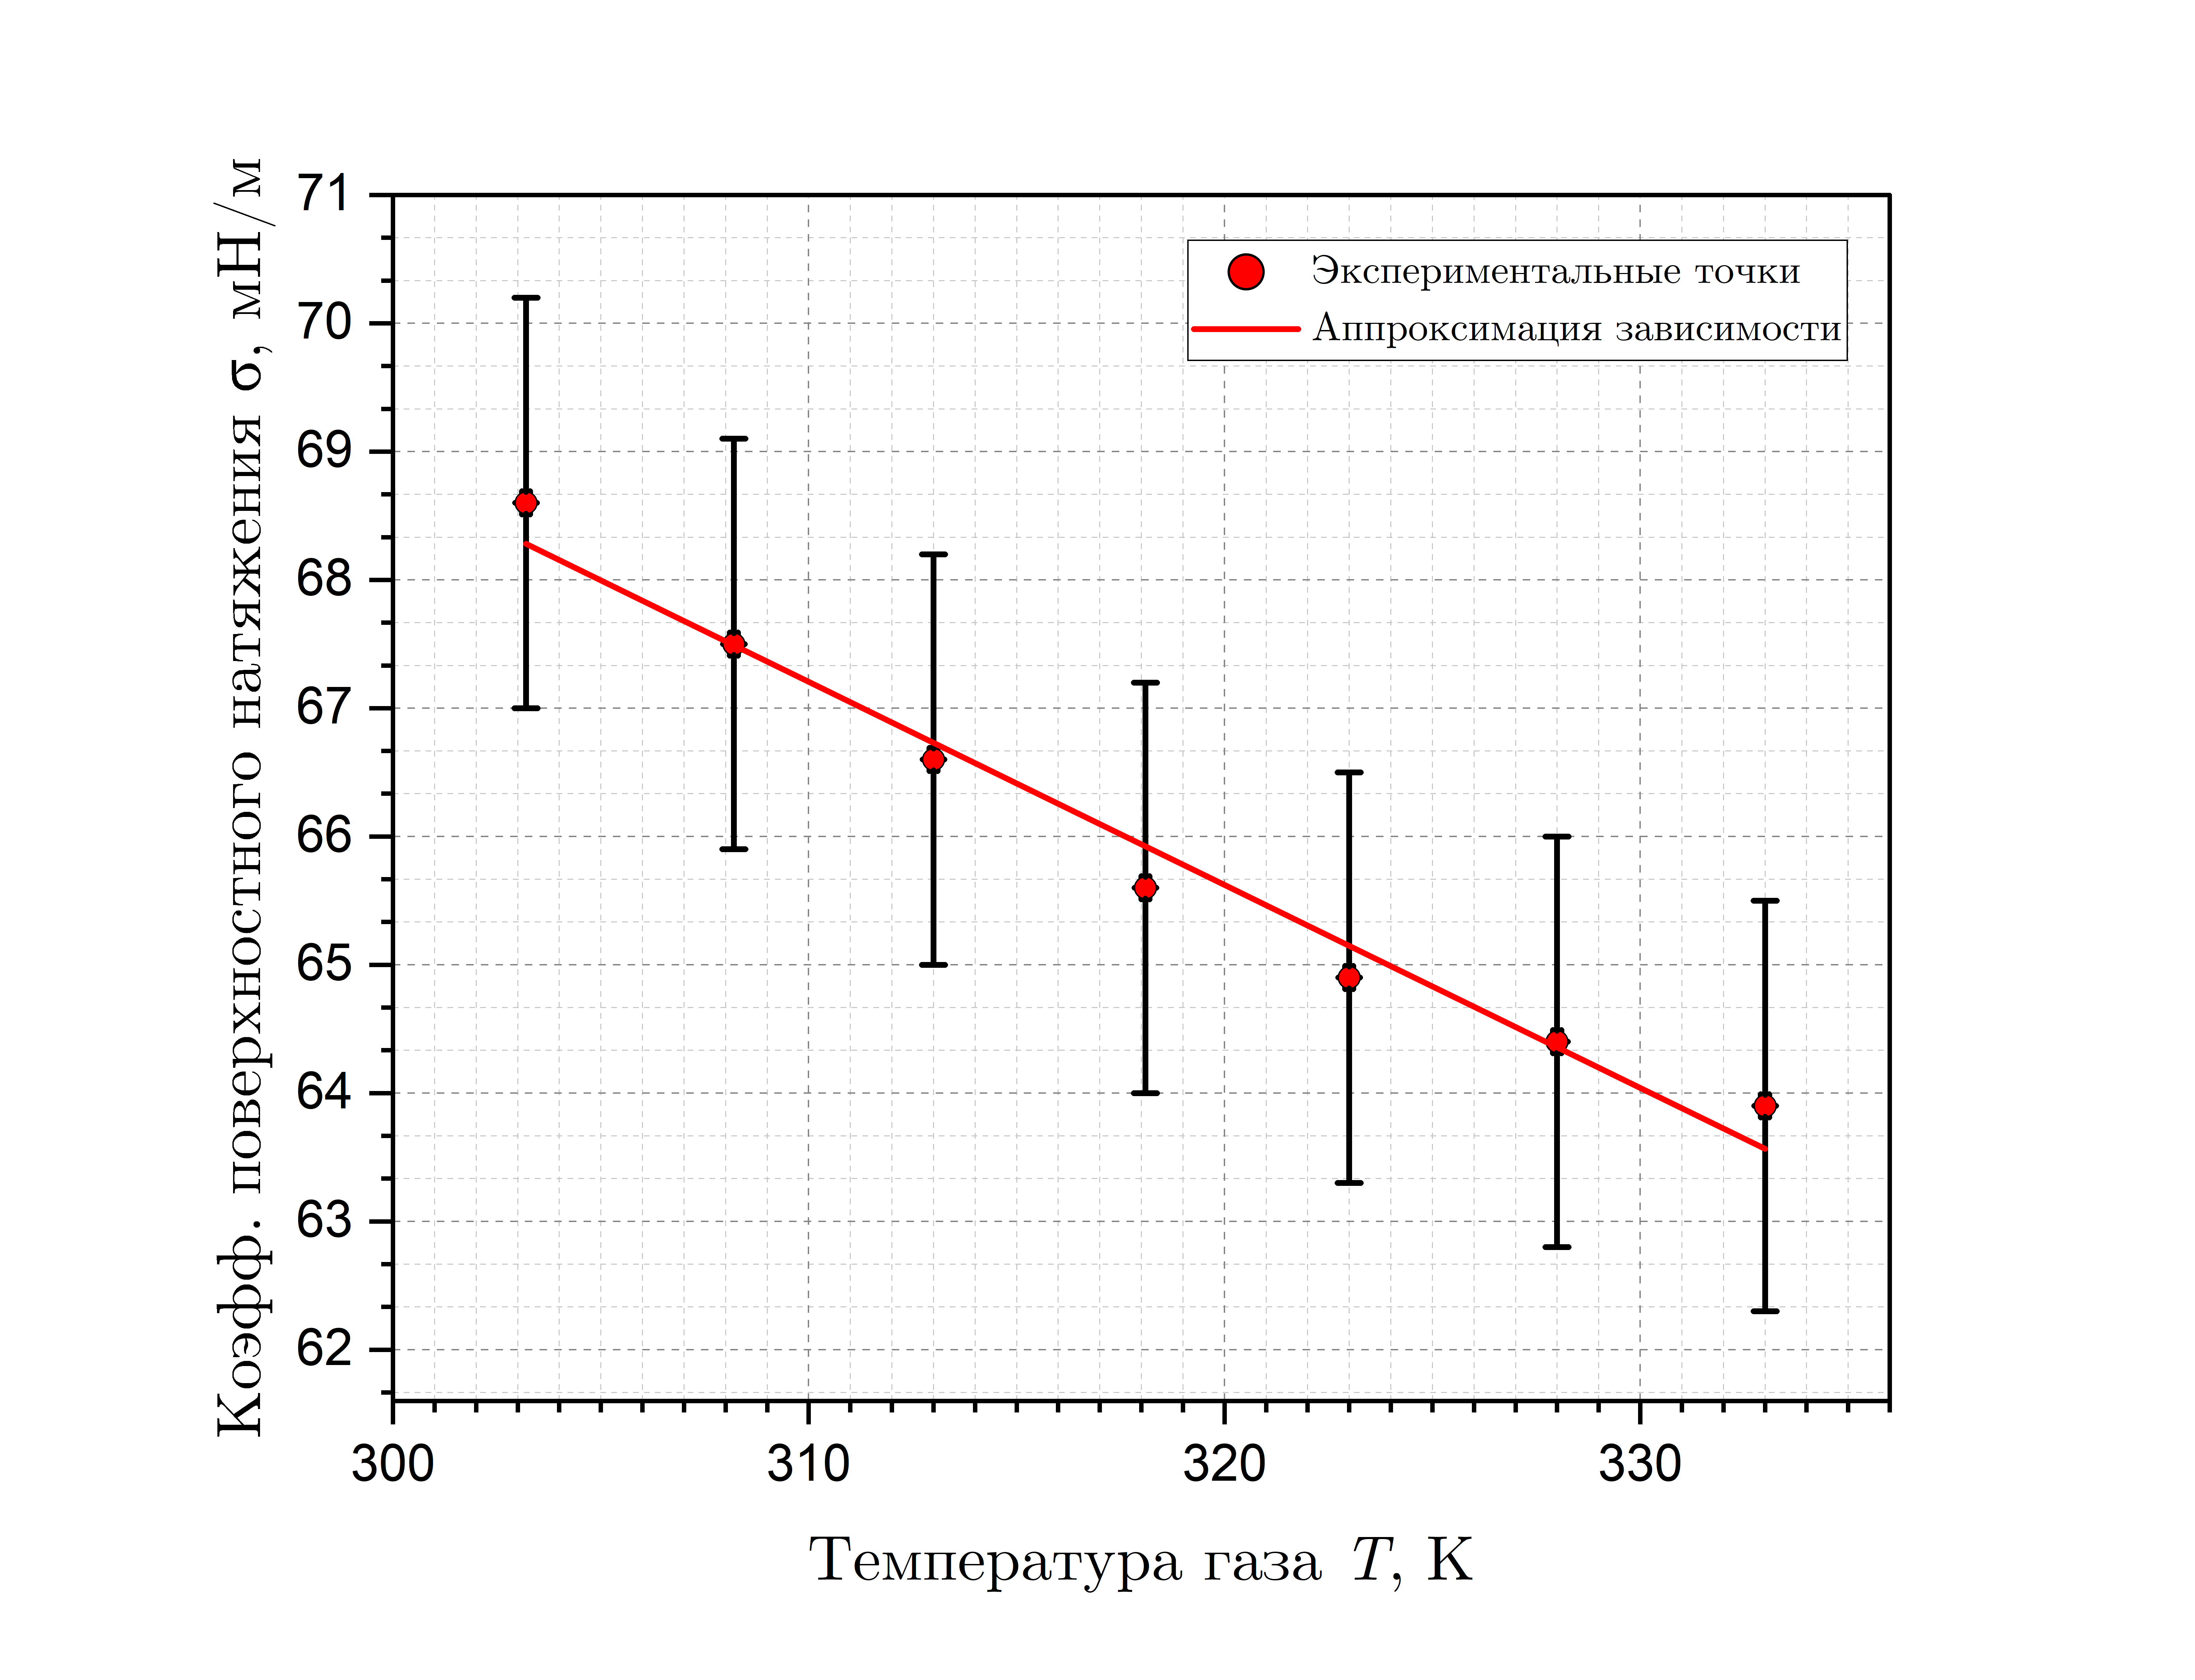
\includegraphics[width=14cm]{images/sigma(T).png}
        \caption{График зависимости коэффициента поверхностного натяжения дистилированной воды $\sigma$ от температуры $T$}
        \label{sigma(T)}
    \end{figure}
    
    \noindent Вычислим коэффициенты аппроксимирующей прямой $\sigma = kT + b$, где $ \displaystyle k = \frac{d\sigma}{dT} $, используя метод наименьших квадратов:

    \[ k = \frac{\langle T\sigma \rangle - \langle T \rangle \langle \sigma \rangle}{\langle T^2 \rangle - \langle T \rangle ^2} \approx -0,158\text{ } \frac{\text{мН}}{\text{м}\cdot\text{К}},\]
    
    \[ b = \langle \sigma \rangle - k\langle T \rangle \approx 116,3\text{ } \frac{\text{мН}}{\text{м}}. \]

    \noindent Полные погрешности измерений определяются следующими соотношениями:
    \[ \sigma_k = \sqrt{(\sigma_k^\text{сист})^2 + (\sigma_k^\text{случ})^2} \approx 0,006 \text{ } \frac{\text{мН}}{\text{м}\cdot\text{К}},\]
    \[ \sigma_b = \sqrt{(\sigma_b^\text{сист})^2 + (\sigma_b^\text{случ})^2} \approx 3,2 \text{ } \frac{\text{мН}}{\text{м}}. \]

    \noindent Таким образом, окончательно получаем:
    \begin{itemize}
            \item $\displaystyle \underline{k = \frac{d\sigma}{dT} = (-0,158 \pm 0,006) \text{ } \frac{\text{мН}}{\text{м}\cdot\text{К}}, \: (\varepsilon = 3,8\%);}$
            \item $\displaystyle \underline{b = (116,3 \pm 3,2) \text{ } \frac{\text{мН}}{\text{м}}, \: (\varepsilon = 2,8\%).}$
    \end{itemize}

    \noindent Дополнительно найдем зависимость теплоты образования единицы поверхности жидкости $q =-T\frac{d\sigma}{dT}$ и поверхностной энергии единицы площади $U/\Pi =\sigma + q$ от температуры. Результаты вычислений представлены в таблице~\ref{table:Graph_2-3}, а графики на рис.~\ref{fig:q(T)} и рис.~\ref{fig:Graph_3}.

    \begin{table}[H]
        \centering
        \begin{tabular}{|c|ccccccc|}
        \hline
        $T$, К  & \multicolumn{1}{c|}{303,2} & \multicolumn{1}{c|}{308,2} & \multicolumn{1}{c|}{313,0} & \multicolumn{1}{c|}{318,1} & \multicolumn{1}{c|}{323,0} & \multicolumn{1}{c|}{328,0} & 333,0 \\ \hline
        $\sigma_T$, К & \multicolumn{7}{c|}{0,1} \\ \hline
        $q$, мДж/${\text{м}}^2$ & \multicolumn{1}{c|}{47,9} & \multicolumn{1}{c|}{48,7} & \multicolumn{1}{c|}{49,5} & \multicolumn{1}{c|}{50,3} & \multicolumn{1}{c|}{51,0} & \multicolumn{1}{c|}{51,8} & 52,6 \\ \hline
        $\sigma_q$, мДж/${\text{м}}^2$ & \multicolumn{1}{c|}{1,8} & \multicolumn{1}{c|}{1,8} & \multicolumn{1}{c|}{1,9} & \multicolumn{1}{c|}{1,9} & \multicolumn{1}{c|}{1,9} & \multicolumn{1}{c|}{2,0} & 2,0 \\ \hline
        $U/\Pi$, мДж/${\text{м}}^2$ & \multicolumn{1}{c|}{116,5} & \multicolumn{1}{c|}{116,2} & \multicolumn{1}{c|}{116,1} & \multicolumn{1}{c|}{115,9} & \multicolumn{1}{c|}{116,0} & \multicolumn{1}{c|}{116,3} & 116,5 \\ \hline
        $\sigma_{U/\Pi}$, мДж/${\text{м}}^2$ & \multicolumn{1}{c|}{4,4} & \multicolumn{1}{c|}{4,4} & \multicolumn{1}{c|}{4,4} & \multicolumn{1}{c|}{4,4} & \multicolumn{1}{c|}{4,4} & \multicolumn{1}{c|}{4,4} & 4,4 \\ \hline
        \end{tabular}
        \caption{Результаты дополнительных вычислений.}
        \label{table:Graph_2-3}
    \end{table}

     \begin{figure}[H]
        \centering
        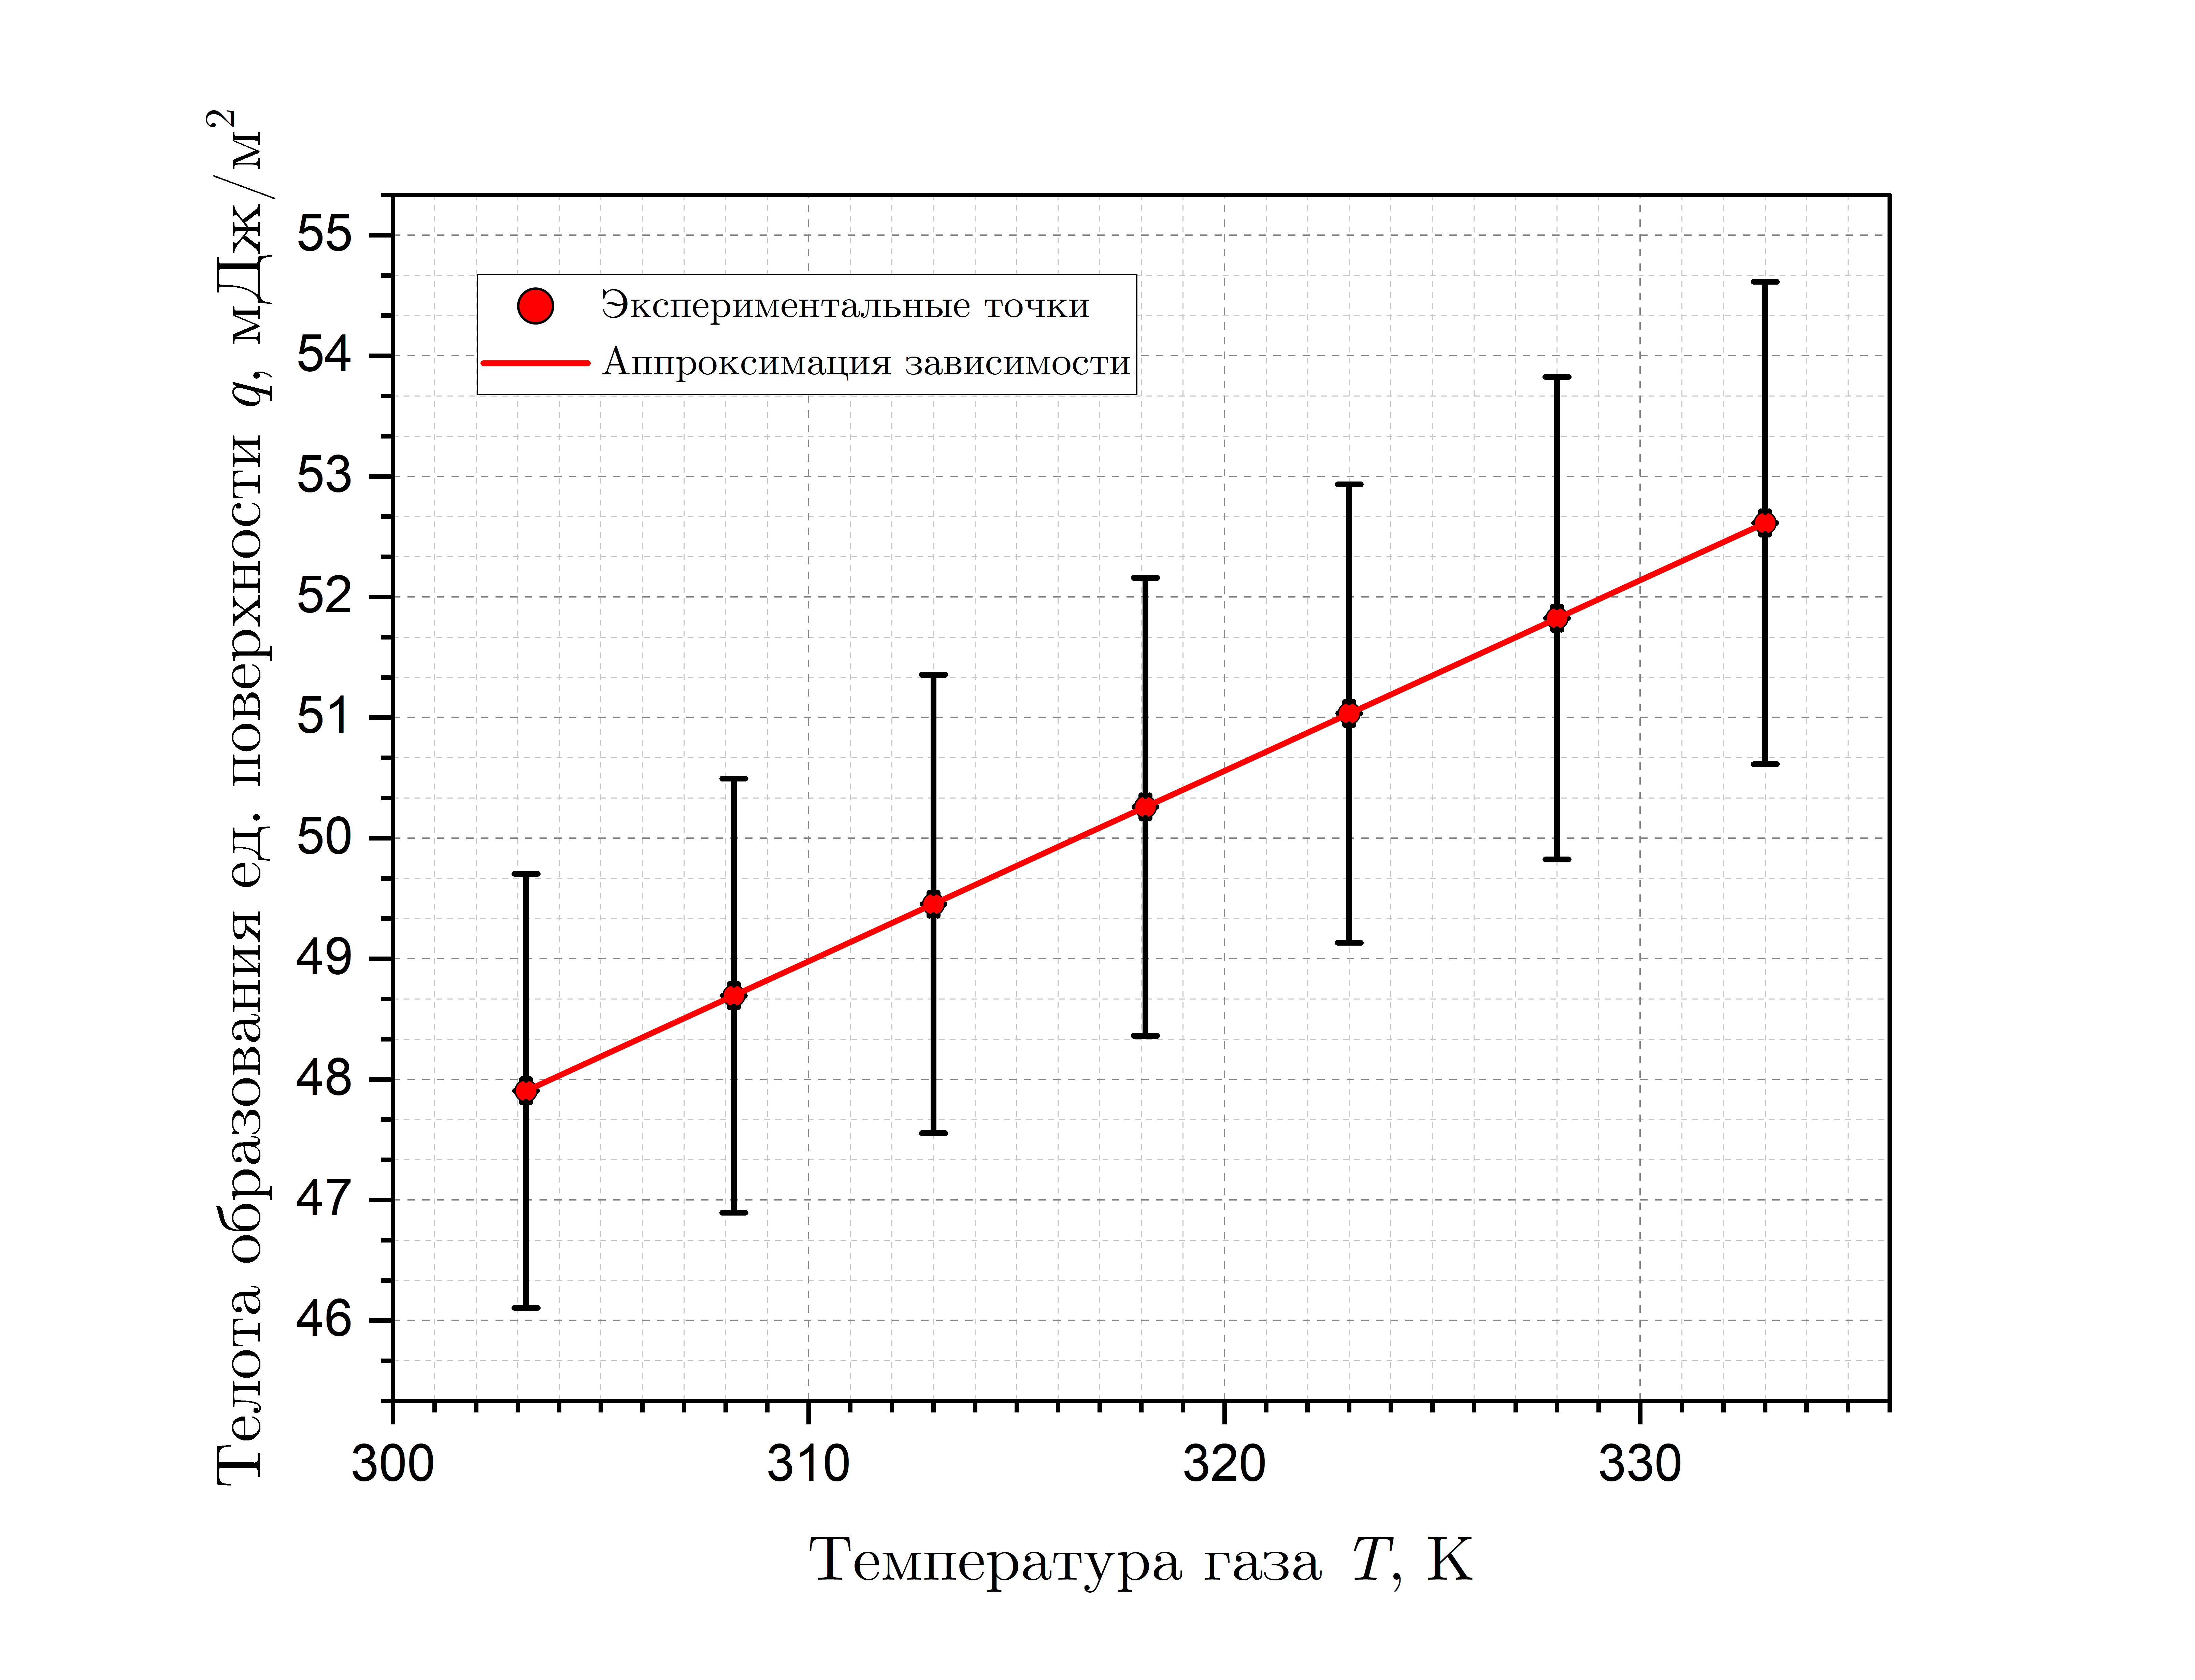
\includegraphics[width=12cm]{images/q(T).png}
        \caption{График зависимости теплоты образования единицы поверхности жидкости $q$ от температуры $T$}
        \label{fig:q(T)}
    \end{figure}
    
    \begin{figure}[H]
        \centering
        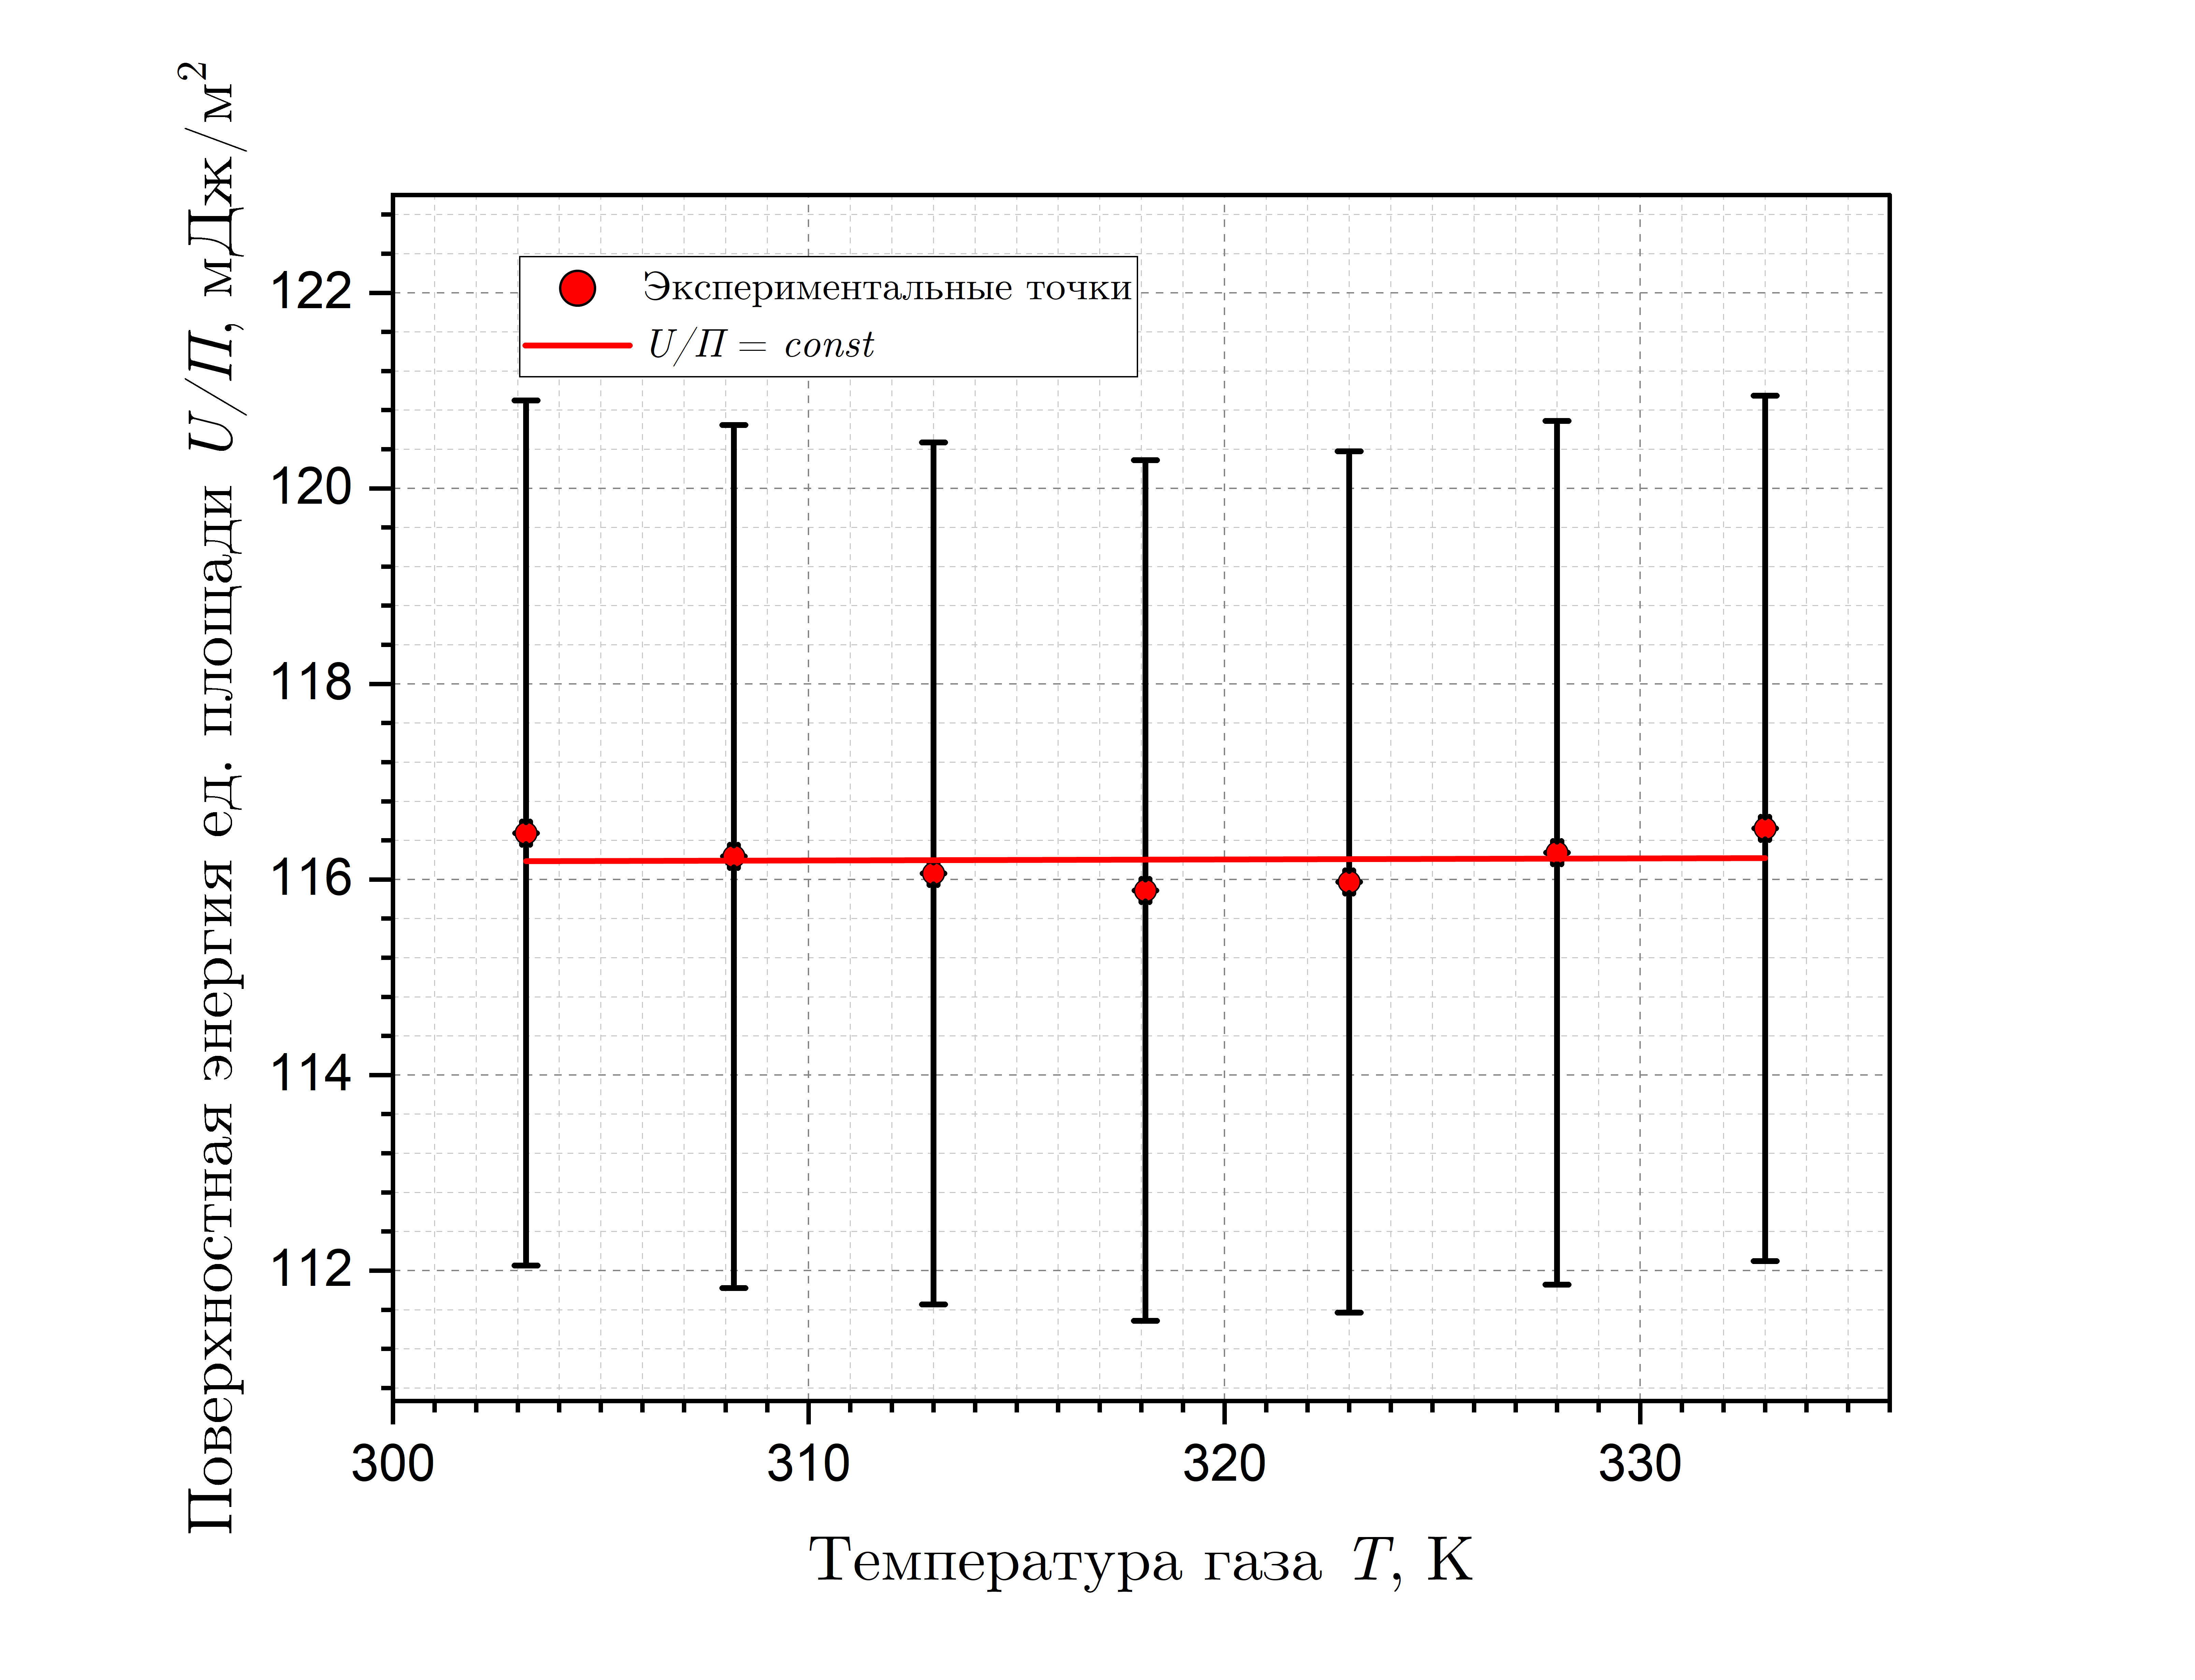
\includegraphics[width=12cm]{images/graph_const.png}
        \caption{График зависимости поверхностной энергии $U$ единицы площади $F$ от температуры $T$}
        \label{fig:Graph_3}
    \end{figure}

    \section*{Заключение}

    В ходе работы были выполнены следующие задачи:
    
    \begin{itemize}
        \item Был измерен диаметр иглы при помощи известного коэффициента поверхностного натяжения спирта. Полученный результат $\underline{ d = (0,99 \pm 0,02) \text{ мм},} \: (\varepsilon = 2,2\%)$ с хорошей точностью совпадает с диаметром, измеренным при помощи светового микроскопа.
    	
        \item Было определено добавочное давление ${\Delta P = (124,4 \pm 2,8) \text{ Па},} \: (\varepsilon = 2,3\%)$, создаваемое столбом жидкости при опускании иглы на ${\Delta h' = (13,0 \pm 0,7) \text{ мм},} \: (\varepsilon = 5,4\%). $ Полученное экспериментально значение $\Delta h$ в пределах погрешности совпало с прямым измерением $\Delta h'$. Полученная поправка к давлению была использована в дальнейшем в основной части работы.
    	
        \item Был экспериментально получен коэффициент поверхностного натяжения воды при различных её температурах. Так, например, при температуре $30^\circ C$ коэффициент $ \sigma \approx (68,6 \pm 1,6) $ мН/м, а при $60^\circ C $ -- $ \sigma \approx (63,9 \pm 1,6) $ мН/м.
    	
        \item Была экспериментально получена зависимость коэффициента поверхностного натяжения дистиллированной воды от температуры. Был вычислен коэффициент пропорциональности, который с учётом погрешности совпал с табличным значением:
        $$\boxed{k = \frac{d\sigma}{dT} = (-0,158 \pm 0,006) \text{ } \frac{\text{мН}}{\text{м}\cdot\text{К}},} \: (\varepsilon = 3,8\%).$$
    	
        \item Были построены графики зависимости от температуры теплоты образования единицы поверхности жидкости и поверхностной энергии единицы площади.
    \end{itemize}
    
    \noindent Полученные результаты дают основание полагать, что теоретические данные довольно точно описывают наблюдаемые зависимости. При этом полученные коэффициенты поверхностного натяжения дистиллированной воды отличаются от табличных данных, что может говорить о низкой точности метода измерений, которая, вероятно, связана с необходимостью учёта сложных не квазистатических процессов, происходящих при пробулькивании пузырька. Также большую погрешность мог внести тот факт, что <<дистиллированная>> вода, используемая в ходе эксперимента имела примеси спирта, которые попали туда в результате некачественной очистки иглы от остатков этанола после первой части работы.  

\end{document}